\chapter{Wstęp}
\label{cha:wstep}

W dzisiejszym czasach z każdej strony otaczają nas różnego rodzaj konstrukcje mechaniczne. Wysokie koszty materiałów skłaniają inżynierów do szukania sposobów na mniejsze ich zużycie oraz zwiększenie żywotności konstrukcji. Dodatkowo pojawia się problem bieżącego sprawdzania stanu konstrukcji w trakcie jej eksploatacji. Jednym ze sposobów badania stanu konstrukcji jest zastosowanie fal mechanicznych. Fale te stały się przedmiotem zainteresowania badaczy już w XIX w. i zaczęły powstawać pierwsze prace takich inżynierów i naukowców jak Poisson, Stokes, Rayleigh. Badania te stawały się popularniejsze i w kolejnych dziesięcioleciach powstawały nowe poważne prace na ten temat. W ostatnich latach pojawiło się duże zainteresowanie wokół tematu fal prowadzonych, które dają duże możliwości badania konstrukcji, ale ich opis jest trudny i najczęściej problemy z nimi związane nie są możliwe do rowiązania w sposób analityczny.

Na gruncie badań nad falami wyłoniły się dwa obszary ich zastosowań tj. badania nieniszczące oraz monitorowanie zdrowia konstrukcji. W pierwszym przypadku celem jest wyszukiwanie uszkodzeń konstrukcji przy pomocy wyspecjalizowanej, przenośnej aparatury poprzez korzystanie z wysokoczęstotliwościowych fal (fal objętościowych). Konstrukcję bada się w różnych punktach, szukając uszkodzenia w bliskim otoczeniu punktu badawczego. Utrudnieniem jest brak odniesienia do wyników poprawnie działającej konstrukcji. Powoduje to, że badania może być bardzo czasochłonne, co podnosi dodatkowo koszty.

Monitorowanie zdrowia konstrukcji skupia się wokół sprawdzania przydatności konstrukcji do użycia i pozostałego czasu, w którym może być ona używana. Możliwe jest to dzięki badaniu z jednego punktu dużego obszaru konstrukcji za pomocą fal prowadzonych. O takich falach mówimy kiedy ich długość staje się porównywalna do wymiarów geometrycznych konstrukcji. Zastosowanie takiego rozwiązania pozwala zautomatyzować proces testowania i zmniejszyć koszta. Aby to było możliwe niezbędne są dane zebrane na prawidłowo działającej konstrukcji. Dodatkowo wymagane jest zastosowanie metod kompensacji zjawisk fizycznych jak dyspersja. Na rysunku \ref{fig:badania_falami} przedstawiony jest sposób badania konstrukcji przy pomocy fal objętościowych oraz fal prowadzonych.

\begin{figure}[h]
\centering
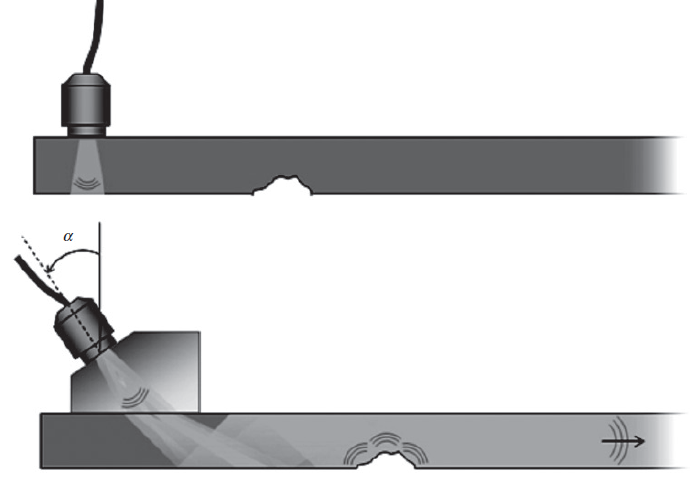
\includegraphics[width=10cm]{Zdjecia/1/badania_falami}
\caption{Przykład badania przy pomocy fal objętościowych (góry rysunek) oraz fal prowadzonych (dolny rysunek)}
\label{fig:badania_falami}
\end{figure}

\section{Cele pracy}
\label{sec:cel}


Praca skupia się wokół symulacji badania metalowych prętów przy pomocy fal prowadzonych. Symulacja ma za zadanie wyznaczyć sygnał zwrotny, dla nadanego sygnału za pomocą np. przetwornika piezoelektrycznego, w przypadku badania puls-echo. Fale prowadzone podlegają dyspersji, więc sygnał powrotny jest silnie zniekształcony w stosunku do nadanego. Algorytmy, które pozwolą skompensować dyspersję są kolejnym aspektem branym pod uwagę przy symulowaniu przebiegu sygnału.

Pomysł na tego typu symulację wziął się z problemu badania kotw stropowych przedstawionego w \cite{kotwy}. Jeśli wykorzystamy metalowe pręty aby wzmocnić strop tunelu i mamy do nich dostęp wyłącznie od strony czoła, to możliwości sprawdzania stanu tych prętów jest mocno ograniczony. Rysunek \ref{fig:kotwy} przedstawia widok tunelu i kotw stropowych. Sposobem na diagnostykę kotw, może być właśnie zastosowanie fal prowadzonych. 

Aby dać możliwość symulacji badania pręta, program musi zapewniać następujące funkcjonalności:
\begin{enumerate}
  \item Możliwość wyboru sygnału wejściowego
  \item Możliwość wyznaczenia modelu matematycznego pręta
  \item Możliwość wyznaczenia sygnału zwrotnego z uwzględnieniem parametrów pręta
  \item Możliwość wyznaczenia krzywych dyspersji dla pręta o zadanych właściwościach materiałowych
  \item Możliwość kompensacji dyspersji sygnału wyjściowego kilkoma, wybranymi metodami.
\end{enumerate}

\vspace{5mm}

Dodatkowo program daje możliwość wyznaczania krzywych wzbudzalności dla pręta i symulacji badania w układzie samowzbudnym (efekt sing-around).





















\section{Plan pracy}
\label{sec:plan_pracy}

Praca podzielona jest na 6 rozdziałów. W rozdziale 1 przedstawiono krótki wstęp oraz założenia projektowe. W rozdziale 2 opisane są podstawowe pojęcia dotyczące propagacji fali w środowisku sprężystym. Podano definicję naprężenia oraz odkształcenia oraz opisano rodzaje fal sprężystych. Następnie przytoczone są informację o zjawisku dyspersji. Opisano przykład kiedy możliwe jest analityczne wyznaczenie krzywych dyspersji oraz przykład gdzie nie jest to już możliwe. Na kolejnych stronach znajdują się metody numerycznego wyznaczania tych krzywych oraz możliwości wyznaczenia ich w badaniach doświadczalnych. Dwie ostatnie sekcje rozdziału skupione są na możliwościach wyznaczania krzywych wzbudzalności oraz ekefcie sing-around. Rozdział 3 przedstawia zagadnienia metody elementów skończonych, które zostały wykorzystane w aplikacji do obliczania modelu pręta. Opisane są kolejno funkcje kształtu, sposoby ich wyznaczania, obliczanie macierzy mas i sztywności elementu oraz agregacja macierzy globalnych. Dla wyznaczonego modelu przedstawiono kilka sposobów wyznaczenia rozwiązania w postaci przemieszczeń, oraz sposoby estymacji błędów rozwiązania i sprawdzenia czy rozwiązanie jest zbieżne. W rozdziale 4 przedstawiono trzy wybrane metody kompensacji dyspersji, które zostały zaimplementowane w programie. Każda metoda opisana została zarówno od strony teoretycznej jak i praktycznej implementacji numerycznej. Ostatni podrzodział stanowi podsumowanie, porównujące wszystkie omawiane metody. Opisane są tam wady i zalety każdej z nich oraz ich ograniczenia. Rozdział 5 stanowi opis zbudowanej aplikacji oraz opis środowiska programistycznego. Początek rozdziału zawiera instrukcję instalacji i konfiguracji interpretera Python programu PyCharm  który został wykorzystany w projekcie. Znajduje się tam rownież lista wszystkich bibliotek niezbędnych do uruchomienia stworzonej aplikacji. Dalsza część rozdziału zawiera pełny opis działania programu wraz z przytoczonymi przykładami wykorzystania. Opisane są kolejne kroki obliczeń dwóch głównych modułów aplikacji tj. budowania modelu wraz z wyznaczaniem krzywych dyspersji oraz kompensowania dyspersji z użyciem wybranej metody.Dodatkowymi elementami jest możliwość symulowania efektu sing-around z pomocą krzywych wzbudzalności oraz korzystanie z zaimplementowanego graficznego interfejsu użytkownika. Rozdział 6 jest podsumowaniem efektów pracy przy projekcie. Opisano stan zrealizowania założeń oraz podano możliwości rozwoju projektu.

































